\documentclass[boxes,pages]{homework}

\name{Nate Stemen}
\studentid{20906566}
\email{nate.stemen@uwaterloo.ca}
\term{Fall 2020}
\course{Numerical Analysis}
\courseid{AMATH 740}
\hwnum{B}
\duedate{Fri, Sep 25, 2020 5:00 PM}

\hwname{Computational Assignment}

\usepackage{physics}
% \usepackage{cleveref}
\usepackage{listings}
\usepackage{xcolor}
\usepackage{graphicx}
\usepackage{caption}

\definecolor{codegreen}{rgb}{0,0.6,0}
\definecolor{codegray}{rgb}{0.5,0.5,0.5}
\definecolor{codepurple}{rgb}{0.58,0,0.82}
\definecolor{backcolour}{rgb}{0.95,0.95,0.92}

\lstloadlanguages{Python}
\lstdefinestyle{mystyle}{
  language=Python,
  backgroundcolor=\color{backcolour},
  commentstyle=\color{codegreen},
  keywordstyle=\color{magenta},
  numberstyle=\tiny\color{codegray},
  stringstyle=\color{codepurple},
  basicstyle=\ttfamily\footnotesize,
  numbers=left,
  numbersep=5pt,
  showstringspaces=false,
  breaklines=true
}
\lstset{style=mystyle}

\begin{document}

\begin{problem}
Implementation of the Gauss-Seidel method.
\end{problem}

\begin{solution}
	First, the code from \verb|GaussSeidel.py|.
	\lstinputlisting[language=Python]{GaussSeidel.py}
	And here's the output of \verb|VerifyGaussSeidel.py|:
	\begin{verbatim}
total error: 7.596379365363873e-14
\end{verbatim}
	So pretty good if I do say so myself.
	And because I'm working in python here's the file \verb|VerifyGaussSeidel.py|.
	\lstinputlisting[language=Python]{VerifyGaussSeidel.py}
\end{solution}

\problemnumber{4}

\begin{problem}
Implementation of the preconditioned CG and GMRES methods.
\end{problem}

\begin{solution}
	First, the code from \verb|myGMRES.py|:
	\lstinputlisting[language=Python]{myGMRES.py}
	\newpage
	Second, the code from \verb|myGMRES_SSOR.py|:
	\lstinputlisting[language=Python]{myGMRESSSOR.py}
	\newpage
	Third, the code from \verb|myCG_SSOR.py|:
	\lstinputlisting[language=Python]{myCGSSOR.py}
	\newpage
	I also wrote a verson of Conjugate Gradient without preconditioning, so here's that:
	\lstinputlisting[language=Python]{myCG.py}
	Now, here's the output of \verb|test_iterative.py|:
	\begin{verbatim}
**********
error for GMRES, # of steps
error: 4.164109009000164e-13
steps: 31
----
error for GMRES_SSOR, # of steps
error: 2.6580413851364233e-12
steps: 22
----
error for CG, # of steps
error: 4.1577704537099615e-13
steps: 31
----
error for CG_SSOR, # of steps
error: 1.904849842831412e-12
steps: 23
----
\end{verbatim}
	And the translated code \verb|test_iterative.py|:
	\lstinputlisting[language=Python]{test_iterative.py}

	\subsection*{(e)}
	Now here's the code for \verb|driverPCG_PGMRES.py|:
	\lstinputlisting[language=Python]{driverPCG_PGMRES.py}
	And it's output:
	\begin{verbatim}
Steps for GMRES:           66
----
Steps for GMRES with SSOR: 31
----
Steps for CG:              66
----
Steps for CG with SSOR:    32
  \end{verbatim}
	And the associated plot.
	\begin{figure}[h]
		\centering
		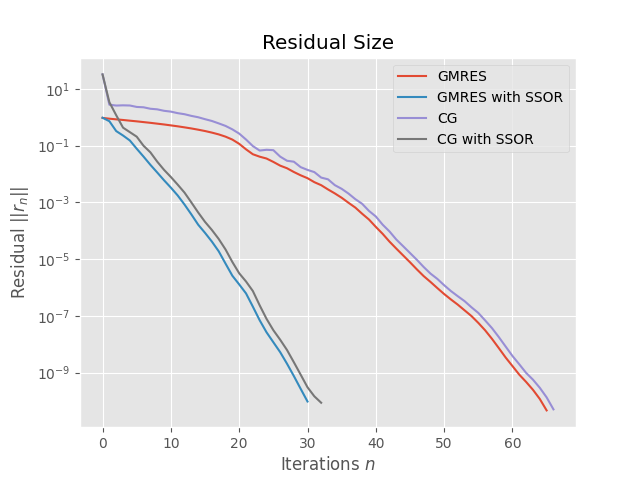
\includegraphics[width=\textwidth]{ressize.png}
		\caption{Residual Size as a function of iteration number}
	\end{figure}
	Really cool to see the two preconditioned algorithms performing so much better on this problem. I would never have expected, but then again, what do I know!? It says in the homework CG with SSOR is the optimal solution for this problem, but GMRES with SSOR seems to be performing slightly better. Why is that?

	\subsection*{(f)}
	For this part I wrote a new file to generate the required log-log plot. Here's \verb|loglog.py|:
	\lstinputlisting[language=Python]{loglog.py}

	This generates the following log-log plot. Note both CG and GMRES (without preconditioning) lie basically on top of each other, and are hard to distinguish.

	\begin{figure}[h]
		\centering
		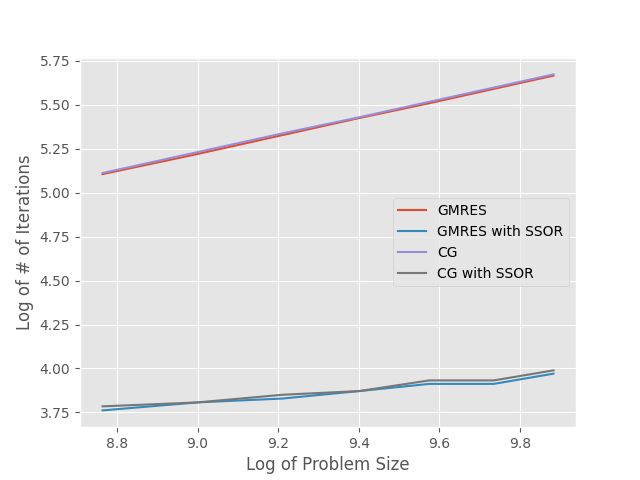
\includegraphics[width=\textwidth]{loglog.png}
		\caption{Log-log plot}
	\end{figure}

	The file also prints out the slopes of these lines as given by \texttt{np.polyfit}.

	\begin{verbatim}
GMRES loglog slope: 0.5013427593113042
CG loglog slope: 0.5003337819405206
GMRES with SSOR loglog slope: 0.17676643756871577
CG with SSOR loglog slope: 0.18072452126753552
\end{verbatim}

	With this we see that both CG and GMRES have a slope of approximately $\frac{1}{2}$ and the preconditioned problems have slope that's about three times as small. Pretty sweet!
\end{solution}

\end{document}